\begin{tikzpicture}
    \node[anchor=north] (img1) at (0,0) {
        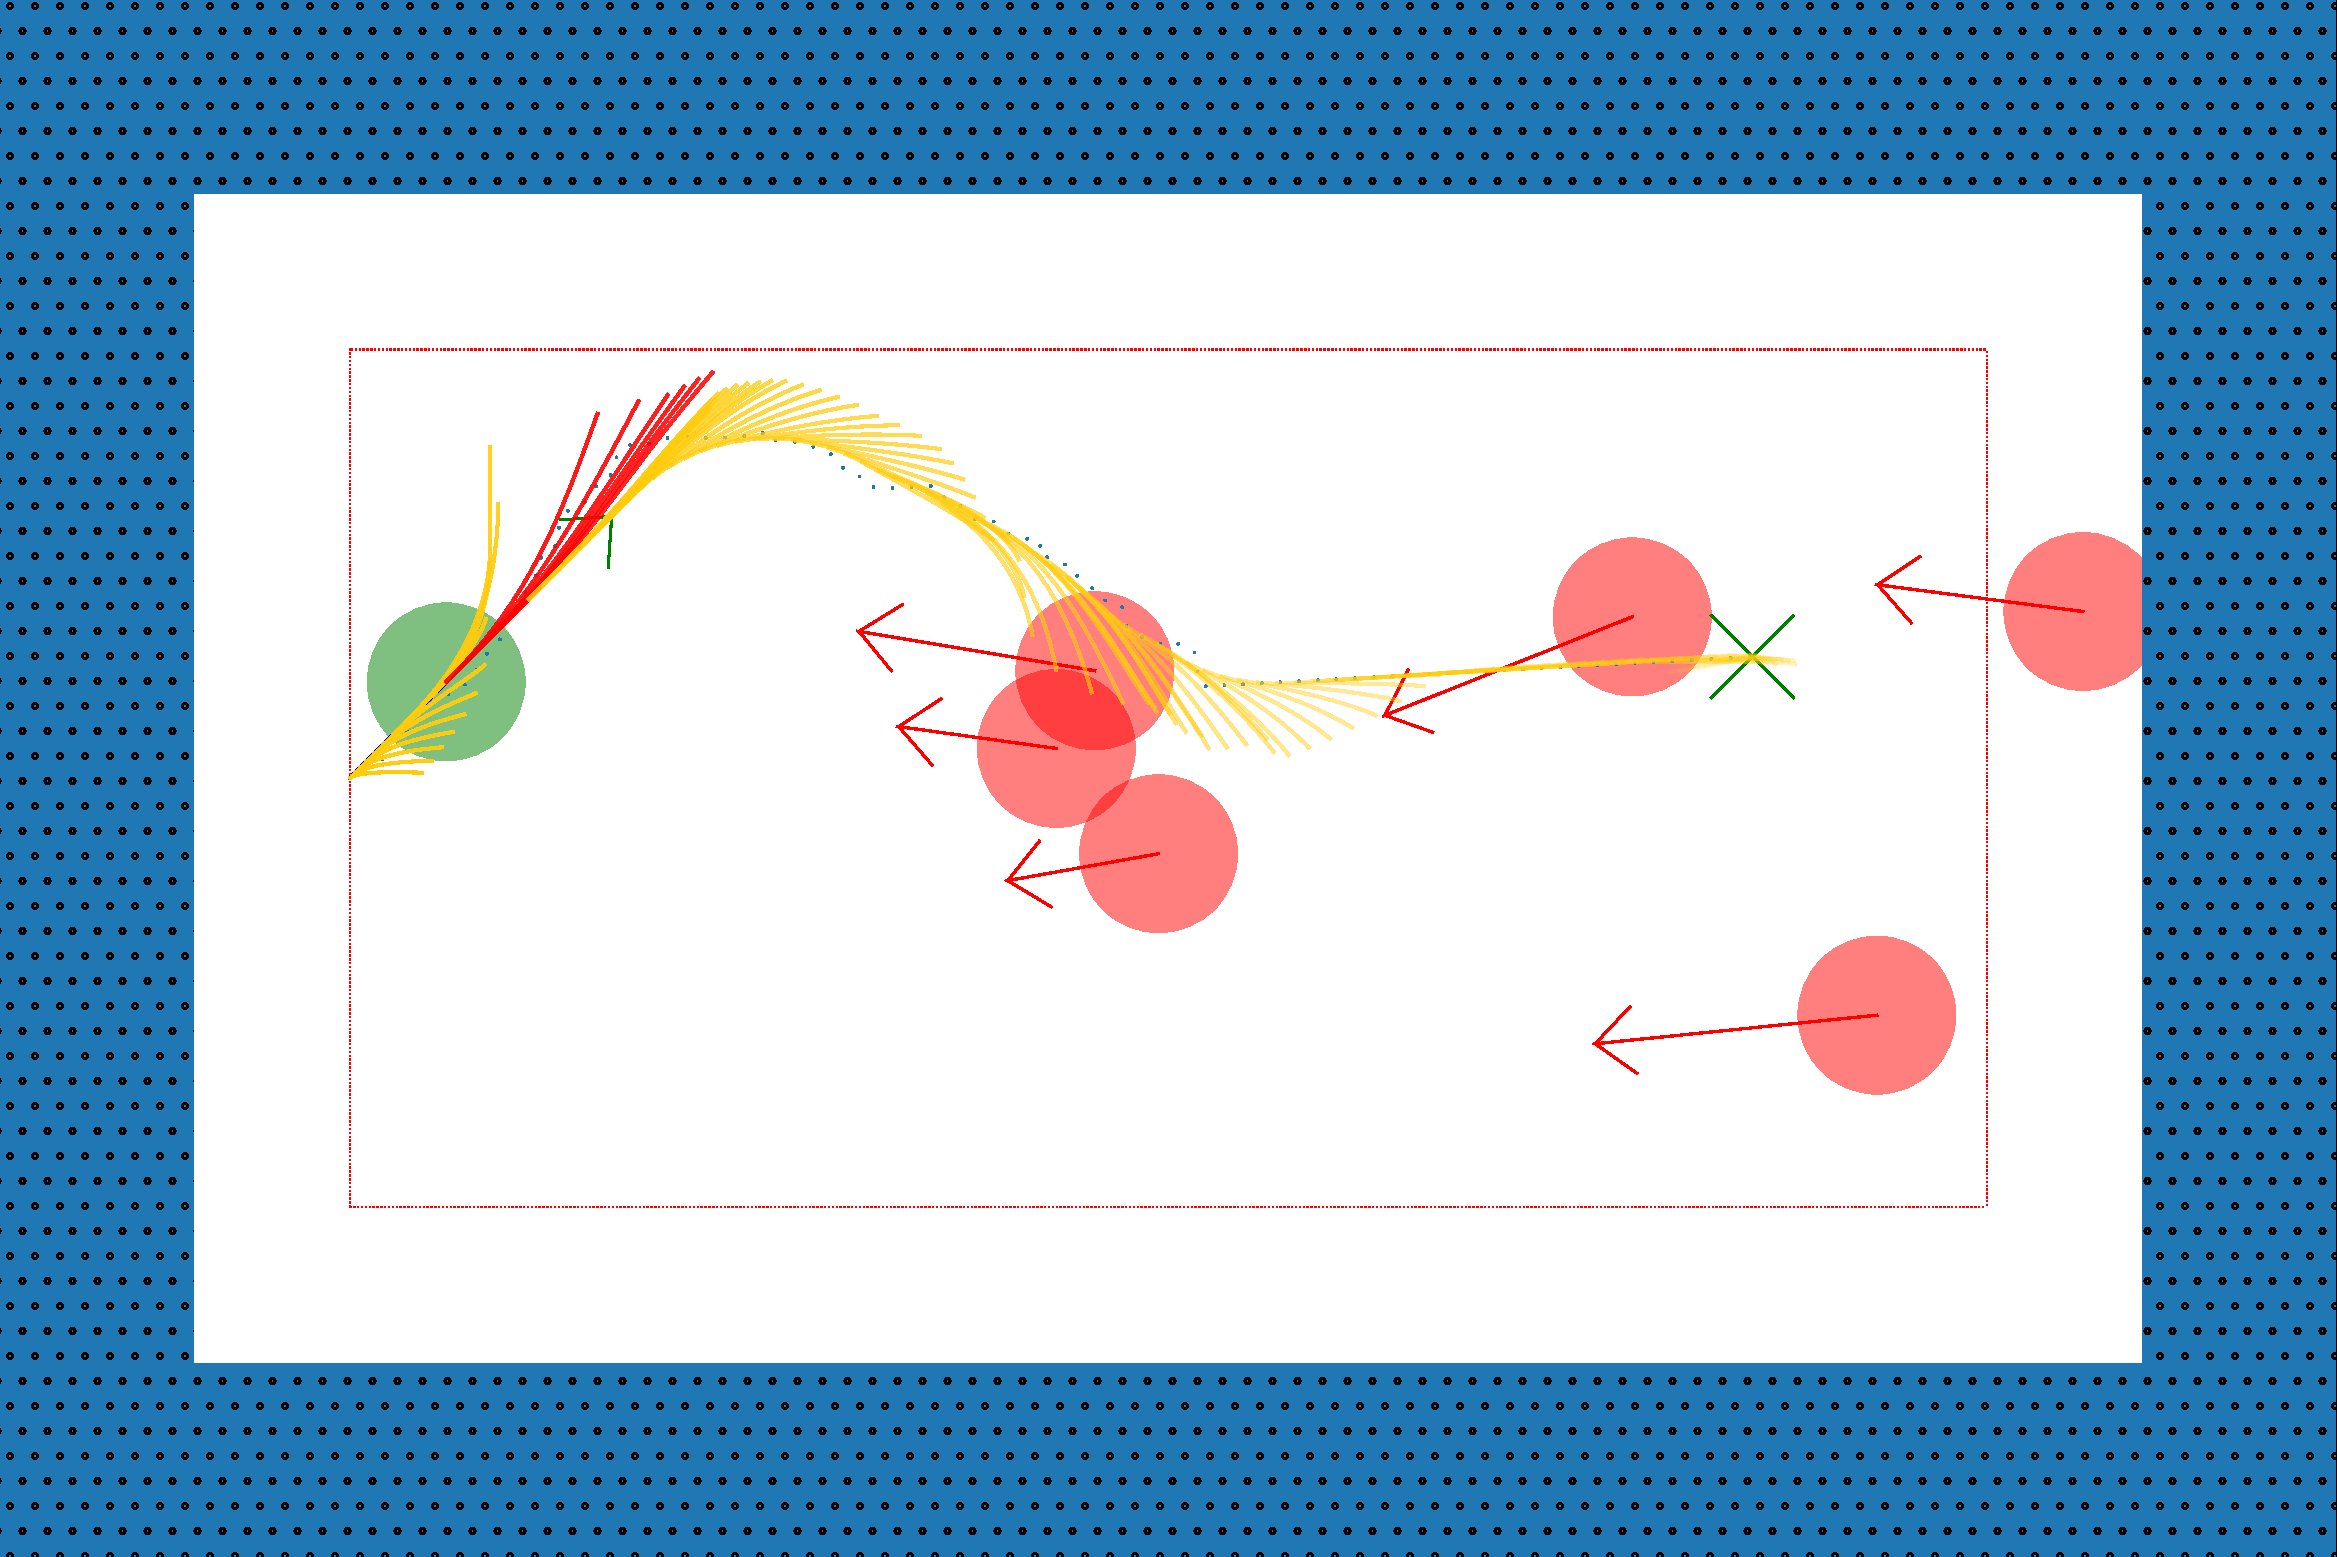
\includegraphics[width=1.\textwidth]{imgs/casc_prob_12.pdf}
    };
    \draw[thick]
        let \p1 = (img1.north east),
            \p2 = (img1.south west),
            \n{w} = {\x1 - \x2},  % width
            \n{h} = {\y1 - \y2}   % height
        in
        (\x2 + 0.151*\n{w}, \y2 + 0.491*\n{h}) rectangle (\x2 + 0.472*\n{w}, \y2 + 0.775*\n{h});

    \node[anchor=north, draw=black, line width=2pt, inner sep=0pt, outer sep=0pt] (img2) at (img1.south) {
        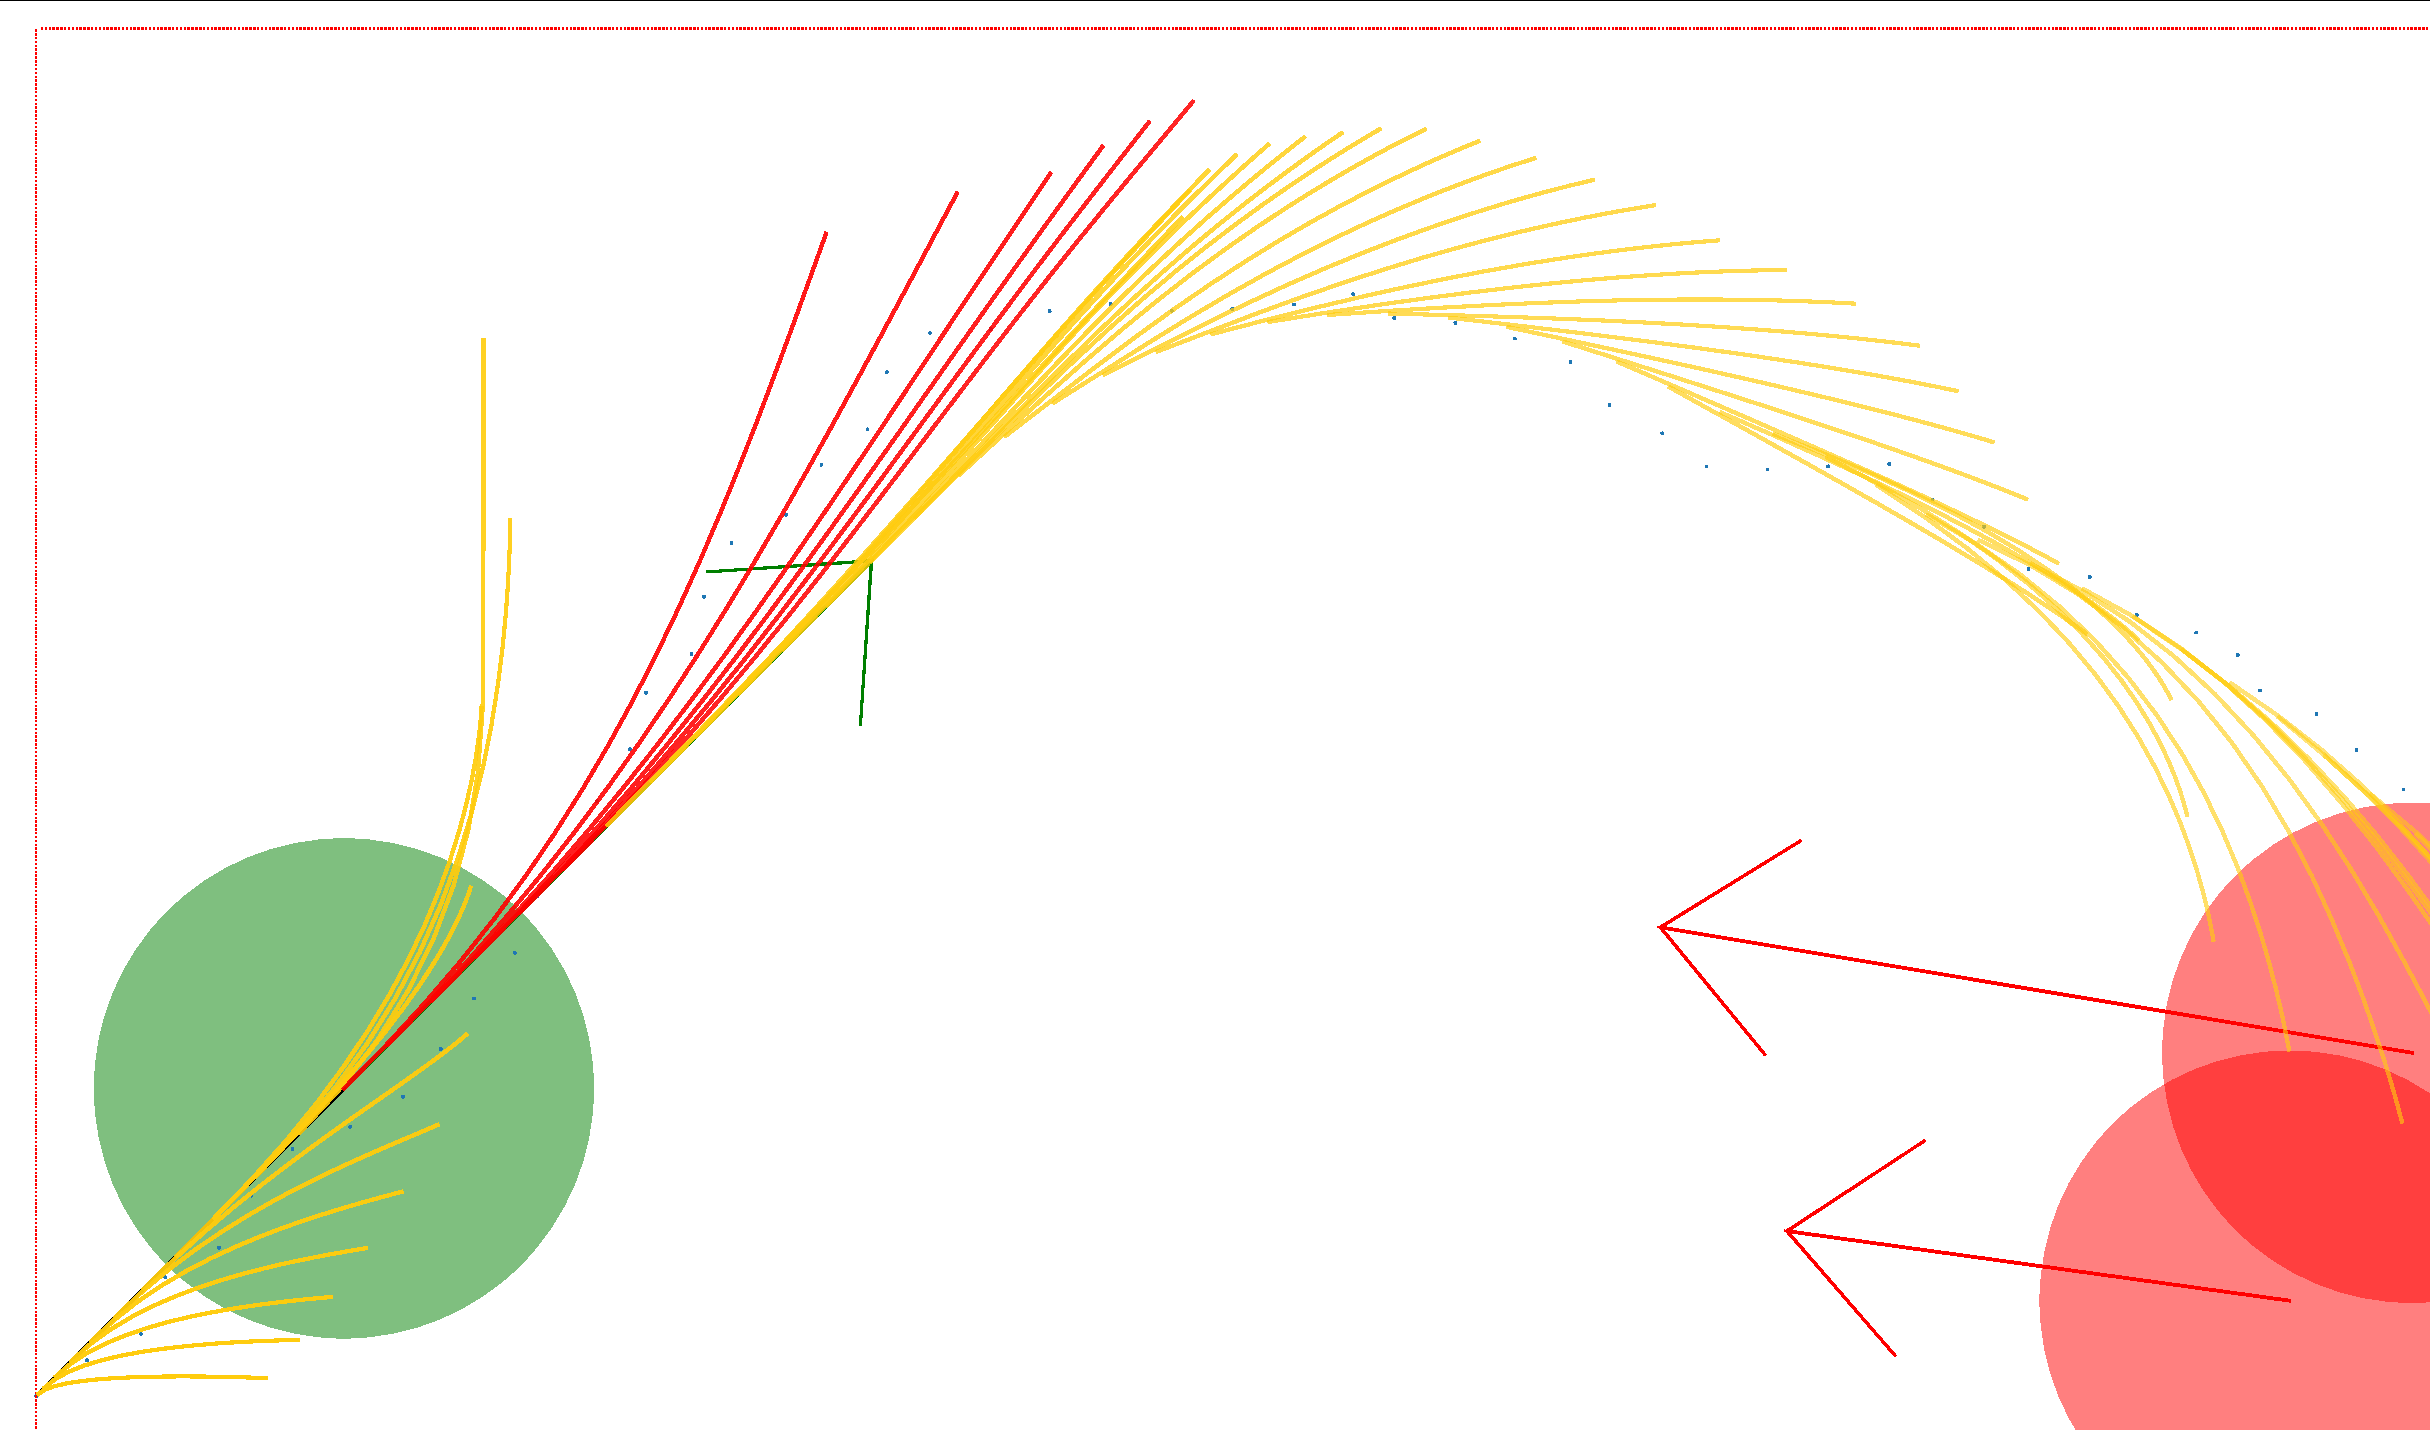
\includegraphics[width=0.95\textwidth]{imgs/casc_prob_12_crop.pdf}
    };
    \draw[thick]
        let \p1 = (img1.north east),
            \p2 = (img1.south west),
            \n{w} = {\x1 - \x2},  % width
            \n{h} = {\y1 - \y2}   % height
        in
        (\x2 + 0.151*\n{w}, \y2 + 0.488*\n{h}) -- ([yshift=0.2mm,xshift=-0.2mm]img2.north west);
    \draw[thick]
        let \p1 = (img1.north east),
            \p2 = (img1.south west),
            \n{w} = {\x1 - \x2},  % width
            \n{h} = {\y1 - \y2}   % height
        in
        (\x2 + 0.47*\n{w}, \y2 + 0.488*\n{h}) -- ([yshift=0.2mm,xshift=0.2mm]img2.north east);
\end{tikzpicture}
